\documentclass[tikz,border=10pt]{standalone}
\usetikzlibrary{positioning, arrows.meta, calc}

\begin{document}
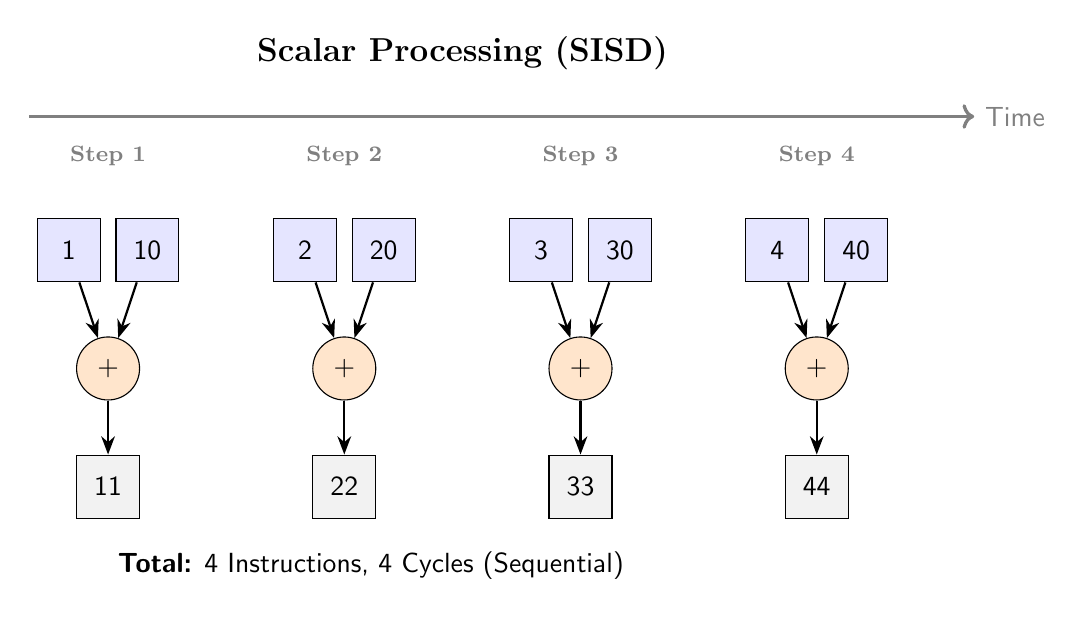
\begin{tikzpicture}[
    node distance=0.8cm,
    font=\sffamily,
    % Styles
    reg/.style={draw, minimum width=0.8cm, minimum height=0.8cm, fill=blue!10, inner sep=0pt},
    op/.style={circle, draw, fill=orange!20, minimum size=0.8cm, inner sep=0pt},
    res/.style={draw, minimum width=0.8cm, minimum height=0.8cm, fill=gray!10, inner sep=0pt},
    arrow/.style={->, >=Stealth, thick},
    label/.style={font=\footnotesize\bfseries, color=gray}
]

    % --- Title ---
    \node[font=\large\bfseries] at (4.5, 2) {Scalar Processing (SISD)};

    % --- TIME AXIS ---
    \draw[->, very thick, gray] (-1, 1.2) -- (11, 1.2) node[right] {Time};

    % --- STEP 1 ---
    \node[label] at (0, 0.7) {Step 1};
    \node[reg] (x1) at (-0.5, -0.5) {1};
    \node[reg] (y1) at (0.5, -0.5) {10};
    \node[op] (add1) at (0, -2) {+};
    \node[res] (r1) at (0, -3.5) {11};

    \draw[arrow] (x1) -- (add1);
    \draw[arrow] (y1) -- (add1);
    \draw[arrow] (add1) -- (r1);

    % --- STEP 2 ---
    \node[label] at (3, 0.7) {Step 2};
    \node[reg] (x2) at (2.5, -0.5) {2};
    \node[reg] (y2) at (3.5, -0.5) {20};
    \node[op] (add2) at (3, -2) {+};
    \node[res] (r2) at (3, -3.5) {22};

    \draw[arrow] (x2) -- (add2);
    \draw[arrow] (y2) -- (add2);
    \draw[arrow] (add2) -- (r2);

    % --- STEP 3 ---
    \node[label] at (6, 0.7) {Step 3};
    \node[reg] (x3) at (5.5, -0.5) {3};
    \node[reg] (y3) at (6.5, -0.5) {30};
    \node[op] (add3) at (6, -2) {+};
    \node[res] (r3) at (6, -3.5) {33};

    \draw[arrow] (x3) -- (add3);
    \draw[arrow] (y3) -- (add3);
    \draw[arrow] (add3) -- (r3);

    % --- STEP 4 ---
    \node[label] at (9, 0.7) {Step 4};
    \node[reg] (x4) at (8.5, -0.5) {4};
    \node[reg] (y4) at (9.5, -0.5) {40};
    \node[op] (add4) at (9, -2) {+};
    \node[res] (r4) at (9, -3.5) {44};

    \draw[arrow] (x4) -- (add4);
    \draw[arrow] (y4) -- (add4);
    \draw[arrow] (add4) -- (r4);

    % Annotations
    \node[below=0.5cm of r2, anchor=west] (desc) at (0, -4) {\textbf{Total:} 4 Instructions, 4 Cycles (Sequential)};

\end{tikzpicture}
\end{document}
